\section{Lược đồ Use-Case - OLD}


\subsection{Use Case cho Người Dùng}
\begin{figure}[H]
    \centering
    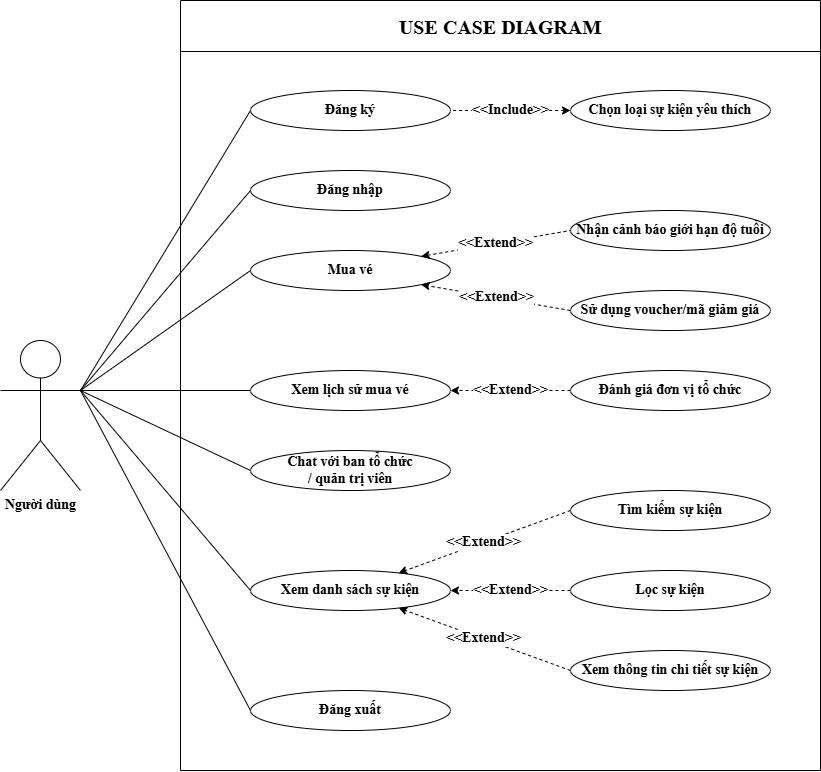
\includegraphics[width=1\textwidth]{Images/User_UseCaseDiagram.png}
    \vspace{10pt}
    \caption{Use Case Diagram -- Người dùng}
    \label{fig:uc_user}
\end{figure}

\subsubsection{Xem, tìm kiếm và lọc thông tin sự kiện}
\begin{table}[H]
\centering
\renewcommand{\arraystretch}{1.3}
\setlength{\tabcolsep}{8pt}
\begin{tabularx}{\textwidth}{|l|X|}
\hline
\textbf{Tên Use Case} & Tìm kiếm và xem thông tin sự kiện \\ \hline
\textbf{Tác nhân} & Người dùng \\ \hline
\textbf{Mục đích} & Giúp người dùng tìm sự kiện theo từ khóa, lọc theo các tiêu chí, xem thông tin chi tiết của sự kiện. \\ \hline
\textbf{Tiền điều kiện} & Không có \\ \hline
\textbf{Hậu điều kiện} & Chi tiết sự kiện phù hợp được hiển thị. \\ \hline
\textbf{Mô tả ngắn gọn} & Người dùng nhập từ khóa và có thể áp dụng bộ lọc (Địa điểm, Ngày diễn ra sự kiện, Giá vé tối thiểu) để tìm kiếm sự kiện; hệ thống trả về kết quả phù hợp, người dùng chọn sự kiện quan tâm để xem chi tiết. \\ \hline
\textbf{Luồng chính} &
1. Người dùng nhập từ khóa vào thanh tìm kiếm trên trang chủ hoặc trang sự kiện. \newline
2. Nếu áp dụng bộ lọc, người dùng có thể lọc theo các tiêu chí: \newline
\hspace*{1em}a) Địa điểm: Thành phố hoặc tỉnh diễn ra sự kiện \newline
\hspace*{1em}b) Ngày diễn ra sự kiện: Những sự kiện có ngày bắt đầu tổ chức nằm trong phạm vi ngày tháng được chọn \newline
\hspace*{1em}d) Giá vé tối thiểu: Giá hạng vé thấp nhất của sự kiện \newline
3. Hệ thống thực hiện truy vấn cơ sở dữ liệu, tìm kiếm sự kiện phù hợp. \newline
4. Hệ thống hiển thị danh sách sự kiện (gồm Poster, Tên, Thời gian, Địa điểm, Giá tối thiểu) theo thứ tự liên quan. \newline
5. Người dùng nhấp vào sự kiện để xem chi tiết. \newline
6. Hệ thống hiển thị: Tên, Poster, địa điểm, ngày tổ chức, mô tả sự kiện, sơ đồ chỗ ngồi hoặc vị trí các hạng vé, giá và số lượng còn lại ứng với các hạng vé hoặc vị trí ghế ngồi, nút mua vé, đơn vị tổ chức (tên, mô tả) và nút chat với Ban tố chức. \newline
7. Người dùng có thể nhấp “Mua ngay” hoặc "Chat vơi Ban tổ chức" để tiếp tục. \\ \hline
\textbf{Luồng thay thế} &
2a. Không tìm thấy kết quả: \newline
\hspace*{1em}Hệ thống hiển thị “Không tìm thấy sự kiện” và gợi ý sự kiện phổ biến hoặc sắp diễn ra. \newline
2b. Sự kiện không còn slot: \newline
\hspace*{1em}Hệ thống hiển thị “Hết vé” và vô hiệu hóa nút mua. \\ \hline
\textbf{Điều kiện lỗi} &
\textbf{Trường hợp lỗi 1:} Truy vấn cơ sở dữ liệu thất bại — Hệ thống hiển thị danh sách sự kiện phổ biến được lưu trữ. \newline
\textbf{Trường hợp lỗi 2:} Thời gian phản hồi quá 3 giây — Hệ thống thông báo “Vui lòng thử lại!”. \\ \hline
\end{tabularx}
\vspace{15pt}
\caption{Đặc tả Use Case -- Xem, tìm kiếm và lọc thông tin sự kiện}
\label{tab:uc_search_event}
\end{table}

\subsubsection{Truy cập chức năng yêu cầu xác thực}

\begin{table}[H]
\centering
\renewcommand{\arraystretch}{1.3}
\setlength{\tabcolsep}{8pt}
\begin{tabularx}{\textwidth}{|l|X|}
\hline
\textbf{Tên Use Case} & Truy Cập Chức Năng Yêu Cầu Xác Thực \\ \hline
\textbf{Tác nhân} & Người dùng \\ \hline
\textbf{Mục đích} & Đảm bảo người dùng đã đăng nhập thành công để truy cập các chức năng cá nhân hóa và nhạy cảm, tránh truy cập trái phép. \\ \hline
\textbf{Điều kiện tiên quyết} &
Người dùng cố gắng thực hiện một trong các chức năng sau: \newline
\hspace*{1em}- Mua vé. \newline
\hspace*{1em}- Xem lịch sử mua vé \newline
\hspace*{1em}- Chat với đơn vị tổ chức sự kiện hoặc quản trị viên. \\ \hline
\textbf{Điều kiện hậu quyết} & Các chức năng được kích hoạt nếu đăng nhập thành công; nếu không, người dùng bị chuyển hướng đến trang đăng nhập. \\ \hline
\textbf{Mô tả ngắn gọn} & Hệ thống kiểm tra trạng thái xác thực (JWT token hoặc session) trước khi cho phép truy cập các chức năng yêu cầu đăng nhập, bao gồm: mua vé, xem lịch sử mua vé và chat với đơn vị tổ chức sự kiện hoặc quản trị viên..\\ \hline
\textbf{Quy trình bình thường} &
1. Người dùng cố gắng truy cập một chức năng yêu cầu đăng nhập (ví dụ: nhấp “Mua vé” hoặc “Vé của tôi”). \newline
2. Hệ thống kiểm tra trạng thái xác thực (JWT token hợp lệ trong localStorage/session). \newline
3. Nếu đã đăng nhập thành công, hệ thống cho phép tiếp tục thực hiện chức năng tương ứng (ví dụ: chuyển đến trang mua vé hoặc hiển thị lịch sử). \newline
4. Hệ thống ghi log truy cập để theo dõi hoạt động. \\ \hline
\textbf{Quy trình thay thế} &
2a. Chưa đăng nhập hoặc token hết hạn: \newline
\hspace*{1em}- Hệ thống hiển thị modal/popup yêu cầu đăng nhập (với liên kết đến trang đăng nhập). \newline
\hspace*{1em}- Người dùng hoàn tất đăng nhập \newline
\hspace*{1em}- Sau khi đăng nhập thành công, hệ thống tự động chuyển hướng trở lại chức năng ban đầu. \\ \hline
\textbf{Điều kiện lỗi} &
- Trường hợp lỗi 1: Token không hợp lệ hoặc bị giả mạo $\rightarrow$ Hệ thống vô hiệu hóa token, ghi log bảo mật và buộc đăng nhập lại. \newline
- Trường hợp lỗi 2: Lỗi kiểm tra xác thực (kết nối backend thất bại) $\rightarrow$ Hệ thống hiển thị “Lỗi hệ thống, vui lòng thử lại” và ghi log để kiểm tra. \\ \hline
\end{tabularx}
\vspace{15pt}
\caption{Đặc tả Use Case -- Truy Cập Chức Năng Yêu Cầu Xác Thực}
\label{tab:uc_auth_access}
\end{table}

\subsubsection{Mua vé}

\begin{table}[H]
\centering
\renewcommand{\arraystretch}{1.3}
\setlength{\tabcolsep}{8pt}
\begin{tabularx}{\textwidth}{|l|X|}
\hline
\textbf{Tên Use Case} & Mua vé sự kiện (bao gồm cảnh báo độ tuổi và áp dụng voucher/mã giảm giá) \\ \hline
\textbf{Tác nhân} & Người dùng \\ \hline
\textbf{Mục đích} & Cho phép người dùng mua vé sự kiện an toàn qua MoMo, đồng thời áp dụng mã giảm giá hay voucher(nếu có) và nhận cảnh báo giới hạn độ tuổi trước khi thanh toán. \\ \hline
\textbf{Điều kiện tiên quyết} &
- Người dùng đã đăng nhập thành công. \newline
- Sự kiện tồn tại, còn slot vé khả dụng. \\ \hline
\textbf{Điều kiện hậu quyết} &
- Thanh toán hoàn tất, vé được cấp thành công. \newline
- Lịch sử mua vé được cập nhật. \\ \hline
\textbf{Mô tả ngắn gọn} &
Người dùng chọn hạng vé, nhận cảnh báo độ tuổi (nếu có), áp dụng voucher hoặc mã giảm giá nếu có và thanh toán qua MoMo QR. \\ \hline
\textbf{Quy trình bình thường} &
1. Người dùng nhấp “Mua vé” từ trang chi tiết sự kiện. \newline
2. Hệ thống kiểm tra trạng thái đăng nhập và slot vé khả dụng. \newline
3. Người dùng chọn hạng vé và số lượng từ sơ đồ ghế hoặc dropdown. \newline
4. Hệ thống kiểm tra nhãn độ tuổi của sự kiện: \newline
\hspace*{1em}- Nếu có giới hạn (P, K, T13, v.v.), hiển thị cảnh báo. \newline
\hspace*{1em}- Người dùng xác nhận tiếp tục hoặc quay lại. \newline
5. Người dùng nhập mã voucher hoặc mã giảm giá (nếu có). \newline
6. Hệ thống xác thực mã voucher hoặc mã giảm giá (kiểm tra tồn tại, còn hiệu lực, áp dụng cho giao dịch). \newline
7. Nếu hợp lệ, hệ thống cập nhật tổng giá vé sau khi giảm. \newline
8. Hệ thống tạo yêu cầu thanh toán và hiển thị mã QR MoMo. \newline
9. Người dùng quét mã QR và hoàn tất thanh toán qua hệ thống MoMo. \newline
10. Hệ thống nhận callback từ MoMo, xác nhận thanh toán, cấp vé (mã QR hoặc ID vé). \newline
11. Hệ thống lưu giao dịch vào lịch sử mua và hiển thị thông báo thành công. \\ \hline
\textbf{Quy trình thay thế} &
4a. Không có giới hạn độ tuổi $\rightarrow$ Bỏ qua bước cảnh báo. \newline
5a. Voucher hoặc mã giảm giá không hợp lệ.
$\rightarrow$ Hệ thống hiển thị cảnh báo không hợp lệ, người dùng có thể nhập mã khác hoặc bỏ qua. \newline
9a. Thanh toán thất bại $\rightarrow$ Hệ thống thông báo “Thanh toán thất bại”, cho phép thử lại hoặc hủy. \\ \hline
\textbf{Điều kiện lỗi} &
- Trường hợp lỗi 1: MoMo API không phản hồi $\rightarrow$ Ghi log và thông báo “Vui lòng thử lại sau 1 phút”. \newline
- Trường hợp lỗi 2: Dữ liệu nhãn độ tuổi không tải được $\rightarrow$ Hệ thống ghi log và cho phép tiếp tục mua vé. \newline
- Trường hợp lỗi 3: Lỗi truy vấn cơ sở dữ liệu voucher/mã giảm giá $\rightarrow$ Hệ thống thông báo “Lỗi hệ thống, vui lòng thử lại”. \\ \hline
\end{tabularx}
\vspace{15pt}
\caption{Đặc tả Use Case -- Mua vé sự kiện}
\label{tab:uc_ticket_purchase}
\end{table}

\subsubsection{Chat với Quản trị viên}
\begin{table}[H]
\centering
\renewcommand{\arraystretch}{1.3}
\setlength{\tabcolsep}{8pt}
\begin{tabularx}{\textwidth}{|l|X|}
\hline
\textbf{Tên Use Case} & Chat với quản trị viên \\ \hline
\textbf{Tác nhân} & Người dùng \\ \hline
\textbf{Mục đích} & Cho phép người dùng giao tiếp với quản trị viên để được hỗ trợ. \\ \hline
\textbf{Tiền điều kiện} & Người dùng đã đăng nhập. \\ \hline
\textbf{Hậu điều kiện} & Tin nhắn được gửi, lịch sử chat được lưu. \\ \hline
\textbf{Mô tả ngắn gọn} & Người dùng khởi tạo chat theo thời gian thực để nhận hỗ trợ. \\ \hline
\textbf{Luồng chính} &
1. Người dùng điều hướng đến trang “Hỗ trợ” (yêu cầu đăng nhập). \newline
2. Hệ thống hiển thị giao diện chat. \newline
3. Người dùng gửi tin nhắn qua WebSocket. \newline
4. Hệ thống lưu tin nhắn vào cơ sở dữ liệu và chuyển đến bàn tổ chức/quản trị viên. \newline
5. Hệ thống thông báo trạng thái gửi thành công. \\ \hline
\textbf{Luồng thay thế} &
3a. Quản trị viên không phản hồi: \newline
\hspace*{1em}1. Hệ thống gửi thông báo “Đang chờ phản hồi”. \newline
\hspace*{1em}2. Người dùng có thể tiếp tục chờ hoặc hủy. \\ \hline
\textbf{Điều kiện lỗi} &
\textbf{Trường hợp lỗi 1:} WebSocket mất kết nối — Hệ thống thử kết nối lại (3 lần). \newline
\textbf{Trường hợp lỗi 2:} Lưu tin nhắn thất bại — Hệ thống thông báo thử lại. \\ \hline
\end{tabularx}
\vspace{15pt}
\caption{Đặc tả Use Case -- Chat với quản trị viên}
\label{tab:uc_chat_admin}
\end{table}

\subsubsection{Chat với Ban tổ chức}
\begin{table}[H]
\centering
\renewcommand{\arraystretch}{1.3}
\setlength{\tabcolsep}{8pt}
\begin{tabularx}{\textwidth}{|l|X|}
\hline
\textbf{Tên Use Case} & Chat với Ban tổ chức \\ \hline
\textbf{Tác nhân} & Người dùng \\ \hline
\textbf{Mục đích} & Cho phép người dùng giao tiếp với Ban tổ chức để được hỗ trợ. \\ \hline
\textbf{Tiền điều kiện} & Người dùng đã đăng nhập. \\ \hline
\textbf{Hậu điều kiện} & Tin nhắn được gửi, lịch sử chat được lưu. \\ \hline
\textbf{Mô tả ngắn gọn} & Người dùng khởi tạo chat theo thời gian thực để nhận hỗ trợ. \\ \hline
\textbf{Luồng chính} &
1. Người dùng chọn chat ngay ở giao diện chi tiết sự kiện hoặc icon chat ở góc màn hình. \newline
2. Hệ thống hiển thị giao diện chat. \newline
3. Người dùng gửi tin nhắn qua WebSocket. \newline
4. Hệ thống lưu tin nhắn vào cơ sở dữ liệu và chuyển đến Ban tổ chức. \newline
5. Hệ thống thông báo trạng thái gửi thành công. \\ \hline
\textbf{Luồng thay thế} &
3a. Ban tổ chức không phản hồi: \newline
\hspace*{1em}1. Hệ thống gửi thông báo “Đang chờ phản hồi”. \newline
\hspace*{1em}2. Người dùng có thể tiếp tục chờ hoặc hủy. \\ \hline
\textbf{Điều kiện lỗi} &
\textbf{Trường hợp lỗi 1:} WebSocket mất kết nối — Hệ thống thử kết nối lại (3 lần). \newline
\textbf{Trường hợp lỗi 2:} Lưu tin nhắn thất bại — Hệ thống thông báo thử lại. \\ \hline
\end{tabularx}
\vspace{15pt}
\caption{Đặc tả Use Case -- Chat với Ban tổ chức}
\label{tab:uc_chat_org}
\end{table}



\subsection{Use Case cho Ban tổ chức}
\begin{figure}[H]
    \centering
    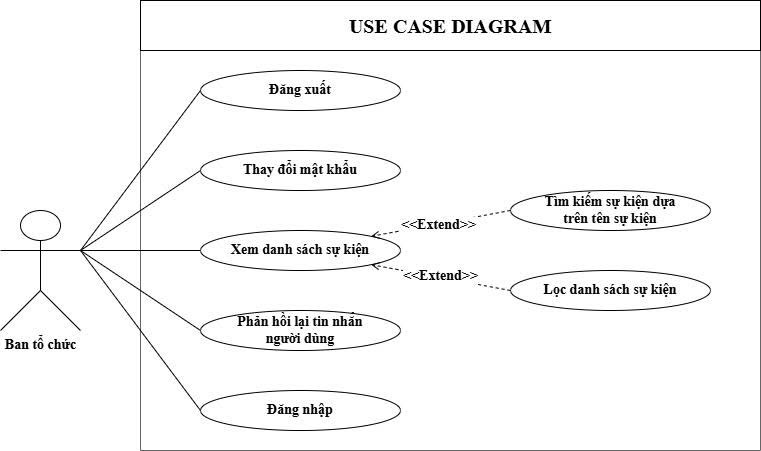
\includegraphics[width=1\textwidth]{Images/Ban_To_Chuc_new.png}
    \vspace{10pt}
    \caption{Use Case Diagram -- Ban tổ chức}
    \label{fig:uc_organizer}
\end{figure}

\subsubsection{Xem, tìm kiếm hoặc lọc danh sách sự kiện}

\begin{table}[H]
\centering
\renewcommand{\arraystretch}{1.3}
\setlength{\tabcolsep}{8pt}
\begin{tabularx}{\textwidth}{|l|X|}
\hline
\textbf{Tên Use Case} & Xem, tìm kiếm hoặc lọc danh sách sự kiện \\ \hline
\textbf{Tác nhân} & Ban tổ chức \\ \hline
\textbf{Mục đích} & 
Cho phép Ban tổ chức xem danh sách sự kiện hiện có, đồng thời hỗ trợ tìm kiếm hoặc lọc sự kiện theo tiêu chí mong muốn (tên, thời gian, trạng thái, đơn vị tổ chức, v.v.). \\ \hline
\textbf{Điều kiện tiên quyết} & 
- Ban tổ chức đã đăng nhập vào hệ thống. \newline
- Cơ sở dữ liệu có thông tin sự kiện. \\ \hline
\textbf{Điều kiện hậu quyết} & 
Danh sách sự kiện hoặc kết quả tìm kiếm/lọc được hiển thị. \\ \hline
\textbf{Mô tả ngắn gọn} & 
Ban tổ chức đăng nhập vào hệ thống để xem danh sách sự kiện. Hệ thống hiển thị toàn bộ hoặc các sự kiện phù hợp với từ khóa/tùy chọn lọc mà Ban tổ chức nhập vào. \\ \hline
\textbf{Quy trình bình thường} &
1. Ban tổ chức đăng nhập thành công vào hệ thống. \newline
2. Hệ thống truy xuất dữ liệu sự kiện trong cơ sở dữ liệu. \newline
3. Hệ thống kiểm tra có sự kiện nào tồn tại không. \newline
4. Nếu có, hệ thống hiển thị toàn bộ danh sách sự kiện. \newline
5. Ban tổ chức nhập từ khóa hoặc tiêu chí lọc (theo tên, thời gian, trạng thái, đơn vị tổ chức, v.v.). \newline
6. Hệ thống tìm kiếm/lọc sự kiện trong cơ sở dữ liệu. \newline
7. Hệ thống hiển thị danh sách kết quả phù hợp. \newline
8. Ban tổ chức chọn một sự kiện cụ thể để xem chi tiết. \newline
9. Sau khi xem xong, Ban tổ chức có thể quay về danh sách sự kiện. \\ \hline
\textbf{Quy trình thay thế} &
3a. Không có sự kiện nào trong cơ sở dữ liệu: \newline
\hspace*{1em}- Hệ thống hiển thị thông báo “Chưa có sự kiện nào.” \newline
6a. Không có kết quả phù hợp với tìm kiếm/lọc: \newline
\hspace*{1em}- Hệ thống hiển thị “Không có sự kiện phù hợp.” \newline
9a. Ban tổ chức không muốn quay lại danh sách sự kiện: \newline
\hspace*{1em}- Hệ thống dừng tiến trình và giữ nguyên trang hiện tại. \\ \hline
\textbf{Điều kiện lỗi} &
- Trường hợp lỗi 1: Lỗi kết nối cơ sở dữ liệu $\rightarrow$ Hệ thống hiển thị “Không thể tải danh sách sự kiện.” \newline
- Trường hợp lỗi 2: Lỗi xử lý truy vấn tìm kiếm/lọc $\rightarrow$ Hệ thống thông báo “Đã xảy ra lỗi, vui lòng thử lại.” \\ \hline
\end{tabularx}
\vspace{15pt}
\caption{Đặc tả Use Case -- Xem, tìm kiếm hoặc lọc danh sách sự kiện (Ban tổ chức)}
\label{tab:uc_view_search_event}
\end{table}

\subsubsection{Phản hồi tin nhắn người dùng}

\begin{table}[H]
\centering
\renewcommand{\arraystretch}{1.3}
\setlength{\tabcolsep}{8pt}
\begin{tabularx}{\textwidth}{|l|X|}
\hline
\textbf{Tên Use Case} & Phản hồi tin nhắn người dùng \\ \hline
\textbf{Tác nhân} & Ban tổ chức \\ \hline
\textbf{Mục đích} & Cho phép Ban tổ chức trả lời tin nhắn do người dùng gửi đến để hỗ trợ, giải đáp hoặc xử lý vấn đề liên quan đến sự kiện. \\ \hline
\textbf{Điều kiện tiên quyết} & 
- Ban tổ chức đã đăng nhập vào hệ thống. \newline
- Có tin nhắn từ người dùng trong danh sách hội thoại. \\ \hline
\textbf{Điều kiện hậu quyết} & 
- Tin nhắn phản hồi được lưu vào cơ sở dữ liệu và gửi đến người dùng. \newline
- Hệ thống hiển thị trạng thái “Đã gửi” cho tin nhắn phản hồi. \\ \hline
\textbf{Mô tả ngắn gọn} & 
Ban tổ chức truy cập mục “Tin nhắn người dùng”, chọn một hội thoại, nhập nội dung phản hồi và gửi tin nhắn. Hệ thống gửi tin nhắn qua WebSocket để đảm bảo tương tác thời gian thực, đồng thời lưu nội dung phản hồi vào cơ sở dữ liệu. \\ \hline
\textbf{Quy trình bình thường} &
1. Ban tổ chức truy cập mục “Tin nhắn người dùng”. \newline
2. Hệ thống hiển thị danh sách hội thoại với người dùng. \newline
3. Ban tổ chức chọn một hội thoại cụ thể. \newline
4. Hệ thống hiển thị nội dung tin nhắn trước đó trong hội thoại. \newline
5. Ban tổ chức nhập nội dung phản hồi và nhấn “Gửi”. \newline
6. Hệ thống gửi tin nhắn qua WebSocket đến người dùng. \newline
7. Hệ thống lưu tin nhắn vào cơ sở dữ liệu. \newline
8. Hệ thống hiển thị trạng thái “Đã gửi”. \newline
9. Nếu người dùng đang trực tuyến, họ nhận được tin phản hồi ngay lập tức. \\ \hline
\textbf{Quy trình thay thế} &
5a. Ban tổ chức không nhập nội dung: \newline
\hspace*{1em}- Hệ thống hiển thị thông báo “Vui lòng nhập nội dung tin nhắn trước khi gửi.” \newline
7a. Mất kết nối WebSocket: \newline
\hspace*{1em}- Hệ thống hiển thị “Kết nối bị gián đoạn, đang thử lại...” và tự động gửi lại tối đa 3 lần. \newline
8a. Lưu cơ sở dữ liệu thất bại: \newline
\hspace*{1em}- Hệ thống hiển thị “Lỗi hệ thống, vui lòng thử lại sau.” \\ \hline
\textbf{Điều kiện lỗi} &
- Trường hợp lỗi 1: Mất kết nối mạng $\rightarrow$ Hệ thống hiển thị “Không thể gửi tin nhắn, vui lòng kiểm tra kết nối.” \newline
- Trường hợp lỗi 2: Tin nhắn không tồn tại hoặc đã bị xóa $\rightarrow$ Hệ thống hiển thị “Tin nhắn không tồn tại.” \newline
- Trường hợp lỗi 3: Lỗi lưu tin nhắn $\rightarrow$ Ghi log hệ thống và thông báo “Vui lòng thử lại sau.” \\ \hline
\end{tabularx}
\vspace{15pt}
\caption{Đặc tả Use Case -- Phản hồi tin nhắn người dùng (Ban tổ chức) }
\label{tab:uc_reply_message}
\end{table}

\underline{Lưu ý:} Đặc tả Use Case cho chức năng phản hồi tin nhắn người dùng trên của Ban tổ chức có thể áp dụng cho vai trò người dùng là quản trị viên trong cùng chức năng.

\subsection{Use Case cho Quản trị viên}
\begin{figure}[H]
    \centering
    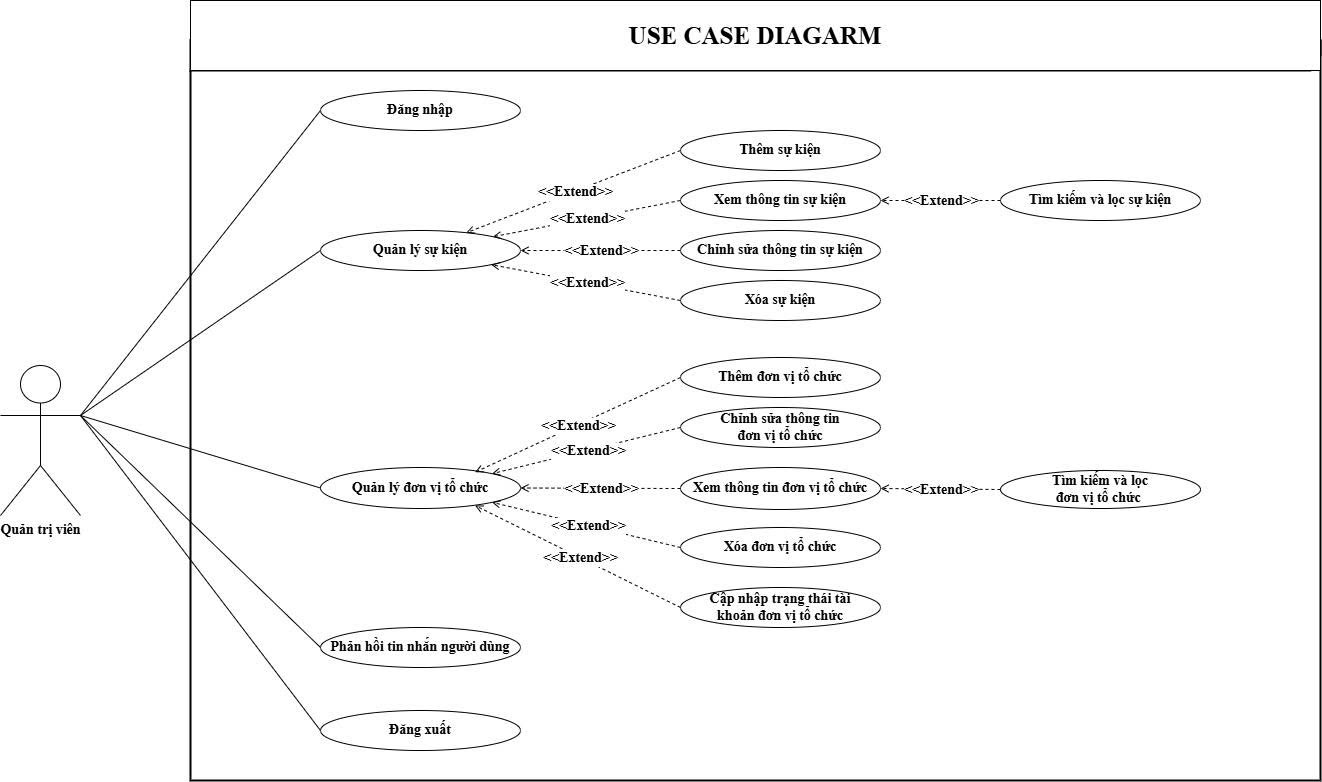
\includegraphics[width=1\textwidth]{Images/Usecase_Admin.jpg}
    \vspace{15pt}
    \caption{Use Case Diagram -- Quản trị viên}
    \label{fig:uc_admin}
\end{figure}

\subsubsection{Quản lý sự kiện}
\begin{table}[H]
\centering
\renewcommand{\arraystretch}{1.3}
\setlength{\tabcolsep}{8pt}
\begin{tabularx}{\textwidth}{|l|X|}
\hline
\textbf{Tên Use Case} & Quản lý sự kiện \\ \hline
\textbf{Tác nhân} & Admin \\ \hline
\textbf{Mục đích} & Quản lý thông tin sự kiện (thêm, sửa, xóa, tìm kiếm). \\ \hline
\textbf{Tiền điều kiện} & Admin đã đăng nhập. \\ \hline
\textbf{Hậu điều kiện} & Thông tin sự kiện được thêm mới, cập nhật hoặc xóa khỏi cơ sở dữ liệu. \\ \hline
\textbf{Luồng chính} &
1. Admin chọn chức năng “Quản lý sự kiện”. \newline
2. Hệ thống hiển thị danh sách sự kiện hiện có. \newline
3. Admin chọn thao tác: thêm, chỉnh sửa, xóa hoặc xem chi tiết sự kiện. \newline
4. Hệ thống xử lý yêu cầu và cập nhật dữ liệu. \\ \hline
\textbf{Luồng thay thế} &
3a. Nếu Admin chọn “Tìm kiếm/Lọc sự kiện”: \newline
\hspace*{1em}a. Hệ thống hiển thị ô tìm kiếm. \newline
\hspace*{1em}b. Admin nhập từ khóa $\rightarrow$ Hệ thống hiển thị danh sách kết quả phù hợp. \\ \hline
\textbf{Điều kiện lỗi} &
1. Nhập thiếu thông tin bắt buộc khi thêm sự kiện $\rightarrow$ Hệ thống báo lỗi và yêu cầu nhập lại. \newline
2. Lỗi hệ thống khi ghi dữ liệu $\rightarrow$ Hệ thống hiển thị thông báo thất bại. \\ \hline
\end{tabularx}
\vspace{15pt}
\caption{Đặc tả Use Case -- Quản lý sự kiện}
\label{tab:uc_manage_event}
\end{table}

\subsubsection{Quản lý đơn vị tổ chức}

\begin{table}[H]
\centering
\renewcommand{\arraystretch}{1.3}
\setlength{\tabcolsep}{8pt}
\begin{tabularx}{\textwidth}{|l|X|}
\hline
\textbf{Tên Use Case} & Quản lý đơn vị tổ chức \\ \hline
\textbf{Tác nhân} & Admin \\ \hline
\textbf{Mục đích} & Quản lý thông tin đơn vị tổ chức (thêm, sửa, xóa, tìm kiếm). \\ \hline
\textbf{Tiền điều kiện} & Admin đã đăng nhập. \\ \hline
\textbf{Hậu điều kiện} & Thông tin đơn vị tổ chức được thêm, cập nhật hoặc xóa khỏi hệ thống. \\ \hline
\textbf{Luồng chính} &
1. Admin truy cập chức năng “Quản lý đơn vị tổ chức”. \newline
2. Hệ thống hiển thị danh sách đơn vị. \newline
3. Admin chọn thao tác: thêm, chỉnh sửa, xóa hoặc xem chi tiết đơn vị. \newline
4. Hệ thống xử lý và lưu kết quả vào cơ sở dữ liệu. \\ \hline
\textbf{Luồng thay thế} &
3a. Nếu Admin chọn “Tìm kiếm/Lọc đơn vị”: \newline
\hspace*{1em}a. Hệ thống hiển thị ô tìm kiếm. \newline
\hspace*{1em}b. Admin nhập từ khóa $\rightarrow$ Hệ thống hiển thị danh sách kết quả phù hợp. \newline
3b. Nếu Admin chọn “Cập nhật trạng thái đơn vị”: \newline
\hspace*{1em}a. Hệ thống hiển thị danh sách trạng thái mới. \newline
\hspace*{1em}b. Admin chọn và lưu thay đổi. \\ \hline
\textbf{Điều kiện lỗi} &
1. Nhập thiếu thông tin bắt buộc khi thêm đơn vị $\rightarrow$ Hệ thống báo lỗi và yêu cầu nhập lại. \newline
2. Lỗi hệ thống khi ghi dữ liệu $\rightarrow$ Hệ thống hiển thị thông báo thất bại. \\ \hline
\end{tabularx}
\vspace{15pt}
\caption{Đặc tả Use Case -- Quản lý đơn vị tổ chức}
\label{tab:uc_manage_organizer}
\end{table}

